% Scenario tree
% Author: Rasmus Pank Roulund
\documentclass{minimal}
\usepackage{tikz}
\usepackage{verbatim}

\begin{comment}
:Title: Scenario tree
:Tags: Trees

A scenario tree from the field of economics. The figure is a replication of a figure 4 from
Barry Eichengreen's NBER paper on "Hegemonic Stability Theories of the International Monetary System" 
from 1987 (PDF_). 

.. _PDF: http://papers.nber.org/papers/W2193.pdf

:Author: Rasmus Pank Roulund

\end{comment}

\usetikzlibrary{shapes}
\usepackage{amsmath}
\usepackage{xspace}
\newcommand{\A}{\ensuremath{\mathcal{A}}\xspace}
\newcommand{\B}{\ensuremath{\mathcal{B}}\xspace}
\newcommand\pa[1]{\ensuremath{\left(#1\right)}}
\begin{document}
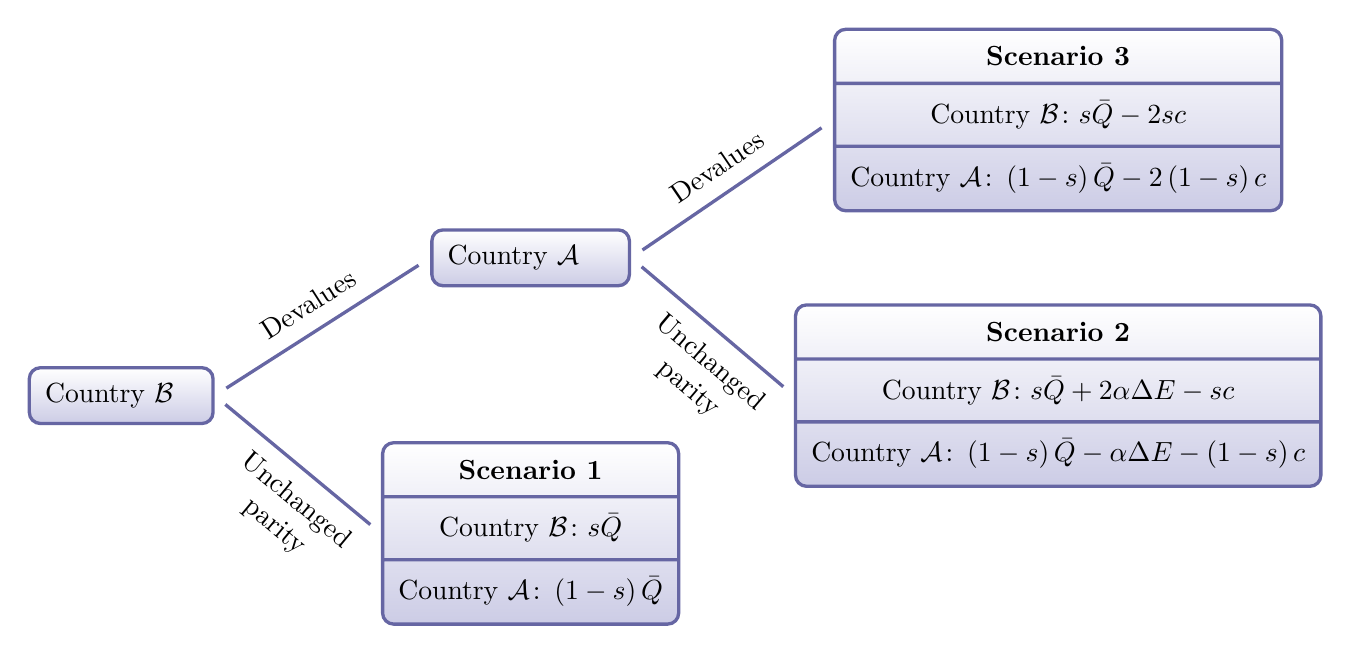
\begin{tikzpicture}[
    grow=right,
    level 1/.style={sibling distance=3.5cm,level distance=5.2cm},
    level 2/.style={sibling distance=3.5cm, level distance=6.7cm},
    edge from parent/.style={very thick,draw=blue!40!black!60,
        shorten >=5pt, shorten <=5pt},
    edge from parent path={(\tikzparentnode.east) -- (\tikzchildnode.west)},
    kant/.style={text width=2cm, text centered, sloped},
    every node/.style={text ragged, inner sep=2mm},
    punkt/.style={rectangle, rounded corners, shade, top color=white,
    bottom color=blue!50!black!20, draw=blue!40!black!60, very
    thick }
    ]

\node[punkt, text width=5.5em] {Country~\B}
    %Lower part lv1
    child {
        node[punkt] [rectangle split, rectangle split, rectangle split parts=3,
         text ragged] {
            \textbf{Scenario  1}
                  \nodepart{second}
            $\text{Country \B}\colon    s\bar{Q}$
                  \nodepart{third}
            $\text{Country \A}\colon\pa{1-s}\bar{Q}$
        }
        edge from parent
            node[kant, below, pos=.6] {Unchanged parity}
    }
    %Upper part, lv1
    child {
        node[punkt, text width=6em] {Country~\A}
        %child 1
        child {
            node [punkt,rectangle split, rectangle split,
            rectangle split parts=3] {
                \textbf{Scenario  2}
                \nodepart{second}
                $\text{Country \B}\colon s\bar{Q}+2\alpha\Delta E -sc$
                \nodepart{third}
                $\text{Country \A}\colon\pa{1-s}\bar{Q}-\alpha\Delta E -
                \pa{1-s}c$
            }
            edge from parent
                node[below, kant,  pos=.6] {Unchanged parity}
        }
        %child 2
        child {
            node [punkt, rectangle split, rectangle split parts=3]{
                \textbf{Scenario 3}
                \nodepart{second}
                $\text{Country \B}\colon s\bar{Q}-2sc$
                \nodepart{third}
                $\text{Country \A}\colon\pa{1-s}\bar{Q}-2\pa{1-s}c$
            }
            edge from parent
                node[kant, above] {Devalues}}
            edge from parent{
                node[kant, above] {Devalues}}
    };
\end{tikzpicture}
\end{document}